\chapter{Configuration functions}
Recall that we defined configuration functions (Definition~\ref{def:config-function}). We begin by proving Theorem~\ref{thm:config-median}.
\begin{proof}
Let $\ov x \in \Omega$, and $\ov\alpha(\ov x)$ be such that
\[
f(\ov x) \leq f(\ov y) + \sqrt{c f(\ov x)} d_{\ov\alpha}(\ov x, \ov y)
\]
Let $S_a = \{\ov y \in \Omega: f(\ov y) \leq a\}$. (Note that in this proof, consider $a$ as the median, which we will substitute later). Then, for $\ov y \in S_a$, 
\begin{align*}
f(\ov x) &\leq f(\ov y) + \sqrt{c f(\ov x)} d_{\ov\alpha}(\ov x, \ov y) \\
\implies f(\ov x) &\leq a + \sqrt{c f(\ov x)} \inf_{\ov y\in S_a} d_{\ov\alpha}(\ov x, \ov y) \\
\implies f(\ov x) &\leq a + \underbrace{\sqrt{c f(\ov x)} \sup_{\ov \alpha: \|\ov\alpha\|=1} \inf_{\ov y\in S_a} d_{\ov\alpha}(\ov x, \ov y)}_{d_T(\ov x, S_a)} \\
\implies d_T(\ov x, S_a) &\geq \frac{f(\ov x) -a}{\sqrt{cf(\ov x)}} \qquad \qquad (*)
\end{align*}
Note that the RHS above is an increasing functions of $f(\ov x)$. If $f(\ov x) \geq a +t$, from $(*)$, we have $d_T(\ov x, S_a) \geq \frac{t}{\sqrt{c}\sqrt{t+a}}$. Thus,
\[
\PP(f(\ov X) \geq a + t) \leq \PP\left(d_T(\ov X, S_a) \geq \frac{t}{\sqrt{c}\sqrt{t+a}}\right)
\]
Also, $\PP(\ov X \in S_a) = \PP(f(\ov X \leq a)$. We get
\[
\PP(f(\ov X) \geq a + t) \PP(f(\ov X) \leq a) \leq \PP(\ov X \in S_a) \PP\left(d_T(\ov X, S_a) \geq \frac{t}{\sqrt{c}\sqrt{t+a}}\right) \leq \exp\left(-\frac{t^2}{4c(t+a)}\right)
\]
The above is implied by Talagrand's inequality. Now use $a = m$ and $a = m-t$ to get the required results (as $\PP(f(\ov X) \leq m)$ and $ \PP(f(\ov X) \geq m) \geq 1/2$.
\end{proof}
Now we prove Theorem~\ref{thm:config-median-2}
\begin{proof}
Let $S_a = \{\ov y \in \Omega: f(\ov y) \leq a\}$. Consider $\ov x \in \Omega$. Then, $\exists \ov \alpha (\ov x) $ such that $\forall \ov y \in S_a$,
\begin{align*}
f(\ov x) &\leq f(\ov y) + cd_{\ov \alpha}(\ov x, \ov y) \\
f(\ov x) &\leq a + c \inf_{\ov y \in S_a} d_{\ov \alpha}(\ov x, \ov y) \\
&\leq a + c \sup_{\ov\alpha:\|\ov\alpha\|=1} \inf_{\ov y \in S_a} f_{\ov \alpha} (\ov x, \ov y) \\
\implies d_T(\ov x, S_a) &\geq \frac{f(\ov x) - a}{c}
\end{align*}
Thus, $f(\ov x) \geq a + t\implies d_T(\ov x, S_a) \geq t/c$. This gives us $\PP(f(\ov x) \geq a + t) \leq \PP(d_T(\ov x, S_a) \geq t/c)$. By definition, $\PP(\ov X \in S_a) = \PP(f(\ov X) \leq a)$.
This gives us,
\[
\PP(f(\ov X) \leq a) \PP(f(\ov X) \geq a + t) \leq \PP(f(\ov X) \in S_a) \PP(f(\ov x) \geq a + t) \leq \PP\left(d_T(\ov x, S_a) \geq \frac tc\right) \leq \exp\left(-\frac{t^2}{4c^2}\right)
\]
Now we can substitute $a = m$ and $a = m-t$ to collectively get $\PP(f(\ov X) \geq m+t)$ and $\PP(f(\ov X) \leq m-t)$, both $\leq 2\exp(-t^2/4c^2)$. Thus gives us via union bound,
\[
\PP(|f(\ov X) - m| \geq t) 4\exp\left(-\frac{t^2}{4c^2}\right)
\]
\end{proof}
\section{Back to Stochastic Traveling Salesman Problem}
We assume that 
\begin{enumerate}
    \item[\circled{1}] the direction doesn't matter for the function value 
    \item[\circled{2}] function value is independent of how the points are indexed
\end{enumerate}
\newcommand{\tsp}{\text{tsp}}
Let $\tsp(\ov x)$ be the minimum length of the traveling salesman tour through the points in $\ov x$. Earlier we had shown that
\[
\PP(\tsp(\ov x) - \beta \sqrt n \geq t\sqrt n) =
\begin{cases}
    \Theta (1) & \text{using BDC} \\
    \exp\left(-\frac{n}{c\log n}\right) &\text{using BMDC}
\end{cases}
\]
Now we will prove an even stronger bound using Talagrand's inequality. \\
Let $\{e_{i,1}, e_{i,2}\}$ be the incoming and outgoing edge into and from $x_i$ in an optimal tour.
\begin{figure}[h]
    \centering
    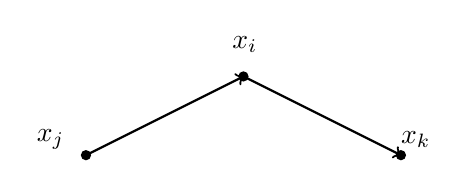
\begin{tikzpicture}
        \draw[thick,fill=black] (0,0) circle (0.5mm);
        \node [left] at (-0.15, 0.2) {$x_j$};
        \draw[thick,fill=black] (4,0) circle (0.5mm);
        \node [left] at (4.5, 0.2) {$x_k$};
        \draw[thick,fill=black] (2,1) circle (0.5mm);
        \node [left] at (2.3, 1.4) {$x_i$};
        \draw[->,thick](0, 0) to (2,1);
        \draw[->,thick](2,1) to (4,0);
    \end{tikzpicture}
\end{figure}
\begin{note}
Fact: $\exists 0 < c < \infty$, such that $\forall n \geq 1$,
\begin{equation}
    \sum_i |e_{i,1}|^2 = \sum_i |e_{i,2}|^2 \leq c
\end{equation}
where $|e_{i,1}|$ is the length of edge $e_{i,1}$.
\end{note}
\begin{prop}
    Let $\beta_k = |e_{k,1}| + |e_{k,2}|$. Then this fact implies that $\sum_{k=1}^n \beta_k^2 \leq 4c$.
\end{prop}
\begin{proof}
\begin{align*}
    (a+b)^2 &\leq 2a^2 + 2b^2 \\
    \therefore, \sum_{k}\beta_k^2 &\leq 2\left(\sum_{k}|e_{k,1}|^2 + \sum_k |e_{k,2}|^2\right) \leq 4c
\end{align*}
\end{proof}
Now think of $\beta_k$ to be the cost of going and coming from point $k$. Large $\beta_k$ means that it is far away from other points. \\
Let $\ov\alpha(\ov x) = \left(\frac{\beta_1}{\|\beta_1\|_2}, \dots, \frac{\beta_n}{\|\beta_n\|_2}\right)$.
\begin{prop}
For any $\ov y \in \Omega$,
\begin{equation}
    \tsp(\ov x) \leq \tsp(\ov y) + d_{\ov \beta} (\ov x, \ov y) \leq \tsp(\ov y) + 2\sqrt{c} d_{\ov \alpha} (\ov x, \ov y)
\end{equation}
\end{prop}
\begin{proof}
Case (i) If $\ov x \cap \ov y = \emptyset$. Then,
\[
d_{\ov\beta}(\ov x, \ov y) = \sum_{i=1}^n \beta_i = 2 \tsp(\ov x)
\]
Then when we substitute , we get 
\[
\tsp(\ov x) \leq \tsp(\ov y) + 2\tsp (\ov x)\text{, which is trivially true}
\]
Case (ii) If $\ov x \cap \ov y \neq \O$. Then, reindexing to align points in $\ov x$ and $\ov y$ reduces the RHS. We wil prove the condition holds for the indexing in which the maximum possible points align.

\end{proof}
\begin{corollary}
\begin{equation}
    \PP\left(|\tsp(\ov X) - m| \geq t\right) \leq 4\exp\left(-\frac{t^2}{16c}\right)
\end{equation}
If $t = \Theta(\sqrt n)$, RHS is $O(\exp(-\widetilde{c} n))$
\end{corollary}
